% $Id$

\chapter{Removing confounds: a classification example}
\label{sec:confounds_clas}
\minitoc

\section{Introduction}

This chapter will describe the steps necessary to remove confounding effects using PRoNTo. Confounds (also known as nuissance variables) are included into predictive variables to improve the statistical significance as well as classification performance. Age, gender or the site where the medical imaging were acquired (in case of a multi-site study) are examples of what can be used to assure that the results obtained are real and not due to other secondary variables.

The dataset used in this chapter can be found in OASIS's website \url{http://www.oasis-brains.org} (data set 1) and consists of a longitudinal collection of 150 subjects aged 60 to 96. Each subject was scanned on two or more visits, separated by at least one year for a total of 373 imaging sessions. For each subject, 3 or 4 individual T1-weighted MRI scans obtained in single scan sessions are included. The subjects are all right-handed and include both men and women. 72 of the subjects were characterized as nondemented throughout the study. 64 of the included subjects were characterized as demented at the time of their initial visits and remained so for subsequent scans, including 51 individuals with mild to moderate Alzheimer’s disease. Another 14 subjects were characterized as nondemented at the time of their initial visit and were subsequently characterized as demented at a later visit. In this example, 95 subjects were selected from OASIS dataset with 56 demented patients and 39 nondemented subjects. Age is considered as the confounds. 

Firstly, we will use PRoNTo to predict if the subject suffers from dementia or not based on MRI scans. We will classify the whole brain images using Support Vector Machines, so the reader is advised to complete the tutorial in Chapter \ref{sec:Block_design_fMRI_dataset} before moving on.
As in previous Chapters, we will start analyzing the data with the PRoNTO's GUI and then repeating the analysis using the {\tt matlabbatch}  system. Please create a folder in your computer to store the results and type

\section{GUI analysis}

We will first analyse the data using PRoNTo's GUI and then repeat the analysis using the {\tt matlabbatch} system. We now start up MATLAB and type `prt' or `pronto' in the MATLAB prompt. This will open the main interface of PRoNTo (see Figure \ref{fig:mainInterface} in Chapter \ref{sec:Block_design_fMRI_dataset}).

%--------------------------------------------------------------------------
\subsection{Data \& Design}

\begin{itemize}
	
	\item In PRoNTo's main window, click on `Data \& Design' and a new window will open, `Data and design' (Figure \ref{fig:dataDesign}). Like in previous chapters, browse the directory in which to save the PRT structure (saved as `PRT.mat'); 
	
	\item In the panel ‘Groups’, click on ‘Add’ and provide a name to the group, e.g. `Dem'. Since in this example we have two groups, it is necessary to add one more called `Non-Dem' after inputting all information about the 'Dem' group;
	
	\item All the images in the dataset correspond to different subjects; therefore, click on the ‘Scans’ tick box. This will lock the ‘Subjects/Scans’ field, allowing you to skip to the third field. See Chapter \ref{sec:Block_design_fMRI_dataset} of the manual for more information on this option; 
	
	\item In the `Modalities' panel, click on `Add' and provide a name to the modality, e.g. `MRI'.
	
	\item Load all the image files belonging the first group. You can select all the files by using the right mouse button and clicking on the option `Select All'. When all the images are selected, click on the `Done' button;
	
	\item In the `Covariates' field, type the covariates you want to regress out. Or you can save all the covariates in a matrix named R and input the full path of this matrix to Covariate. Each variable is a column, hence if there is only one covariate, R is a column vector;if there are multiple variables, R will be a matrix containing multiple columns where each column is a covariate. Users can give this matrix any saving name, but after loading into MATLAB, this matrix should only be R.mat. In this example, `Age' is the confounding factor chosen (Figure \ref{fig:covariates});
	
	\begin{figure}[!h]
	\centering
		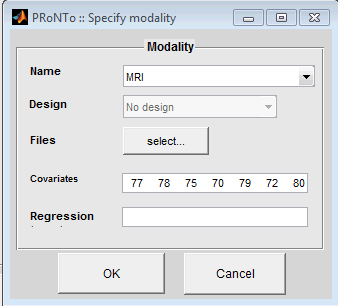
\includegraphics[scale=0.7]{images/Tutorial/confounds/covariates.png}
	\caption{`Specify modality' GUI allows one to enter the covariates to be regressed out.}
	\label{fig:covariates}
	\end{figure}
	
	\item In the `Masks' field, on the bottom left of the `Data and design’ window, select the `mergedsmwrc1\_mask\_01' mask for the modality specified (Figure \ref{fig:mask_cov}). 
	
	\begin{figure}[!h]
	\centering
		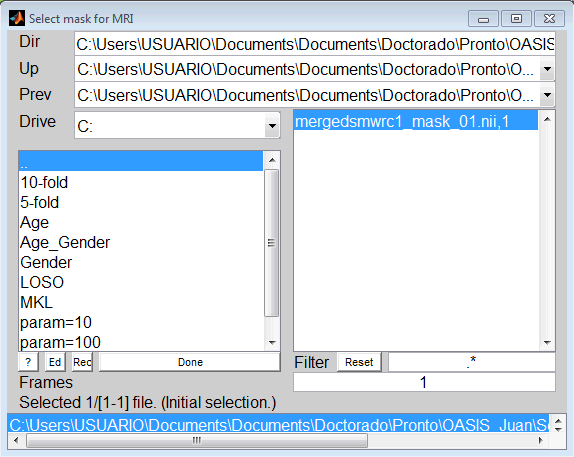
\includegraphics[scale=0.7]{images/Tutorial/confounds/mask_cov.png}
	\caption{This window is called when one clicks `Masks'.}
	\label{fig:mask_cov}
\end{figure}
	
	\item Finally, repeat the previous steps for `Non demented' group, including the corresponding images and covariates, and using the same modality and mask as for `Demented' group. The `Data and design' window should look similar to Figure \ref{fig:data_and_design}. Click on the `Save' button to create `PRT.mat' file with the structure containing the information that has been previously specified. If no errors are shown in the MATLAB command, leave the `Data and design' window by clicking `Quit'.

\begin{figure}[!h]
	\centering
		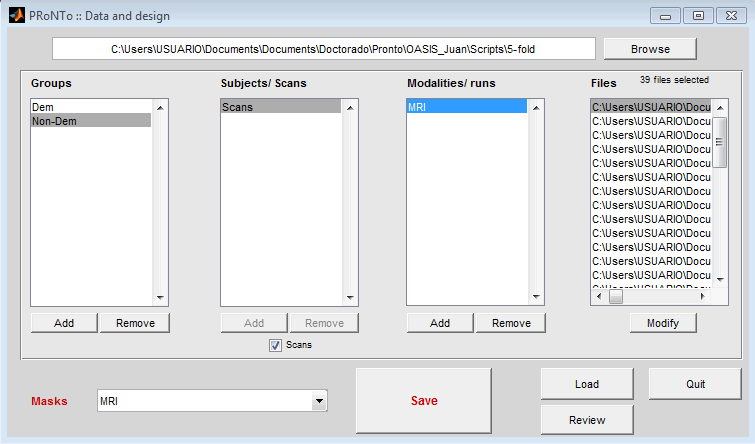
\includegraphics[scale=0.7]{images/Tutorial/confounds/Data_and_design.png}
	\caption{`Data and design' GUI final configuration..}
	\label{fig:data_and_design}
\end{figure}

\end{itemize}

%--------------------------------------------------------

\subsection{Prepare feature set}

\begin{itemize}
	
	\item In PRoNTo's main window, click on `Prepare feature set' and a new window will open, `Prepare feature set' (see Figure \ref{fig:prepareFeature} in Chapter \ref{sec:Block_design_fMRI_dataset});
	\item Select the `PRT.mat' file previously created in the `Data \& Design' step and another window will open, `Specify modality to include' (Figure \ref{fig:specifyModality});

	
	\begin{figure}[!h]
	\centering
		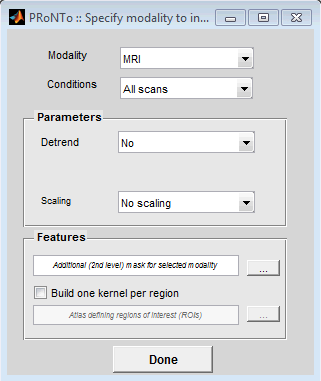
\includegraphics[scale=0.7]{images/Tutorial/confounds/specify_modality.png}
	\caption{`Specify modality to include' GUI.}
	\label{fig:specifyModality}
	\end{figure}
		
	\item In the `Prepare feature set' window, provide a name for the feature set, e.g. `svmDemNonDem';

	\item Click on `Build kernel/data matrix' to build the feature set and kernel.

\end{itemize}



%---------------------------------------------------------------------

\subsection{Specify model}

\begin{itemize}
	
	\item In PRoNTo's main window, click on `Specify model' and a new window will open, `Specify model' (see Figure \ref{fig:specifyModel} in Chapter \ref{sec:Block_design_fMRI_dataset});

	\item Select the `PRT.mat' file and provide a name to the model, e.g. `svm';
	
	\item Select one of the `Feature Set' previously defined. In this case, there is only one:  `svmDemNonDem';
	
	\item Leave the option `Use kernels' tick box as it is, i.e. `Yes';

	\item	Select the `Classification' model type and click on `Define classes` button. A new window will open, `Specify classes' (Figure \ref{fig:classes}), to define the number of classes and a name for each class. We will define 2 classes. For `Class 1' select group `Dem', and all subjects and, similarly, for `Class 2' select group `Non-Dem' and all the subjects from this group.
	
\begin{figure}[!h]
	\centering
		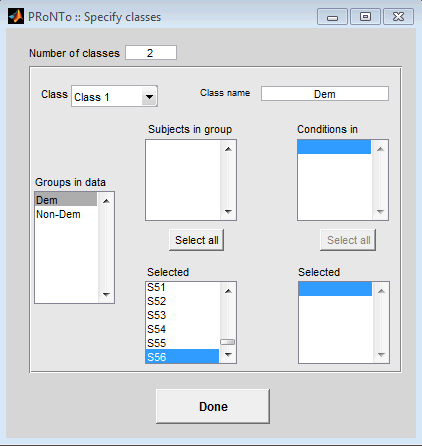
\includegraphics[height=9cm]{images/Tutorial/confounds/classes.png}
	\caption{`Specify classes' GUI.}
	\label{fig:classes}
\end{figure}
	
	\item Select the `Binary support vector machine' option, in the `Machine' field;
	
	\item Leave the option `Optimize hyper-parameter' tick box unchecked and `Cross-Validation Scheme' (internal loop) as it is; 
	
	\item Select the `Leave One Subject Out' cross-validation scheme (external loop);
	
	\item In the `Data operations' box, select the `Regress out covariates (subject level)' option, which corresponds to the removal of the contribution of some external variables to the data, and `Mean centre features using training data' option. Then, the `Specify model' window should look similar to Figure \ref{fig:finalModel}. Click on the `Specify and run model' button;
	
	\begin{figure}[!h]
	\centering
		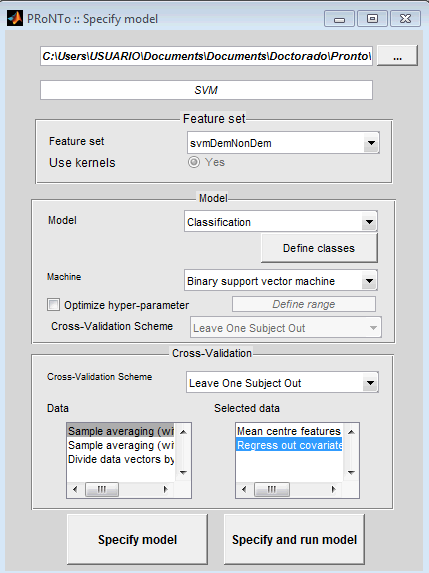
\includegraphics[scale=0.65]{images/Tutorial/confounds/specify_model.png}
	\caption{`Specify model' GUI final configuration.}
	\label{fig:finalModel}
\end{figure}

	
\end{itemize}


%------------------------------------------------------------------

\subsection{Display results}
\label{display_results_confounds}

\begin{itemize}
	
	\item In PRoNTo's main window, click on `Display results' and select the `PRT.mat' file. This will open the main results window (Figure \ref{fig:results});
	
\begin{figure}[h!]
	\centering
		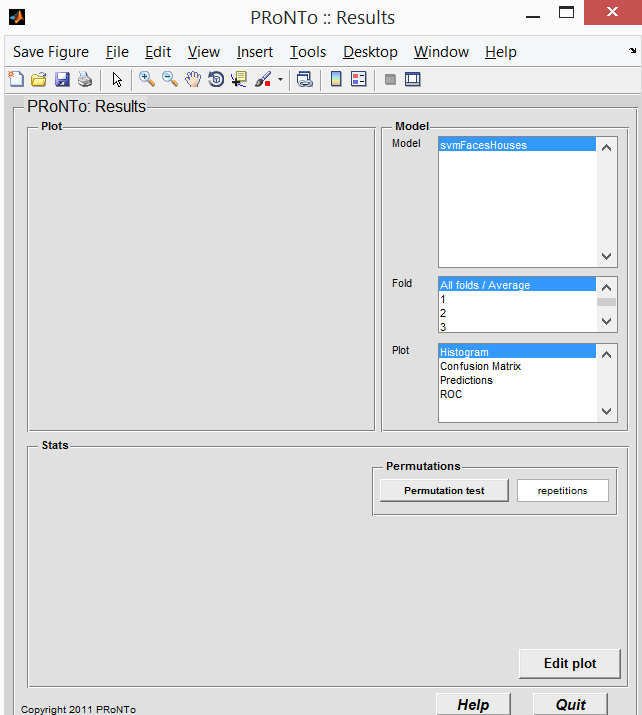
\includegraphics[scale=0.65]{images/Tutorial/confounds/results.png}
	\caption{`Results' GUI.}
	\label{fig:results}
\end{figure}
	
	
	\item In the `Results' window, one can select a different plot in the `Plots' list;

\end{itemize}
	

%=====================================================

\section{Batch analysis}
\label{sec:Batch_analysis_svm_confounds}

In this section, the previous experiment will be repeated using the `\texttt{matlabbatch}' system. The reader is advised to complete the tutorial in Section \ref{sec:Batch_analysis_svm} before continuing, since the explanation of each step will be less descriptive.

Once again, to analyse the data, create a new directory in which to save the results of the analysis. On the main interface of PRoNTo click on the `Batch' button to open the `{\tt matlabbatch}'. Alternatively, type `prt\_batch' in the MATLAB prompt.

%--------------------------------------------------------------

\subsection{Data \& Design}

\begin{itemize}

 	\item Click on `Data \& Design' in the PRoNTo menu (see Figure \ref{fig:batchData} in Chapter \ref{sec:Block_design_fMRI_dataset});	
	\item In the `Directory' field, select a directory where the `PRT.mat' file will be saved;
	
	\item In the `Groups' field:
 	
		\begin{itemize}
		
		\item Add two groups;
		
		\item In the field `Name', provide a name without spaces to both groups, e.g. `Dem' and 'Non-Dem'; 
		
		\item In the field `Select by', select the `Scans' option and add a new modality. For more information on the Scans option please consult Chapter \ref{chap:DataDesign};
		
		\item Add one modality for each subject and provide a name, e.g. `MRI'; and in the field `Scans', select the proper images for each of the groups;	
		
		\item Specify in the `Covariates' the file with the confounds you want to remove. Remember that this file should contain a variable `R' with a matrix of covariates. The batch editor should look similar to the Figure \ref{fig:covariates_batch};
		
		\begin{figure}[h!]
	\centering
		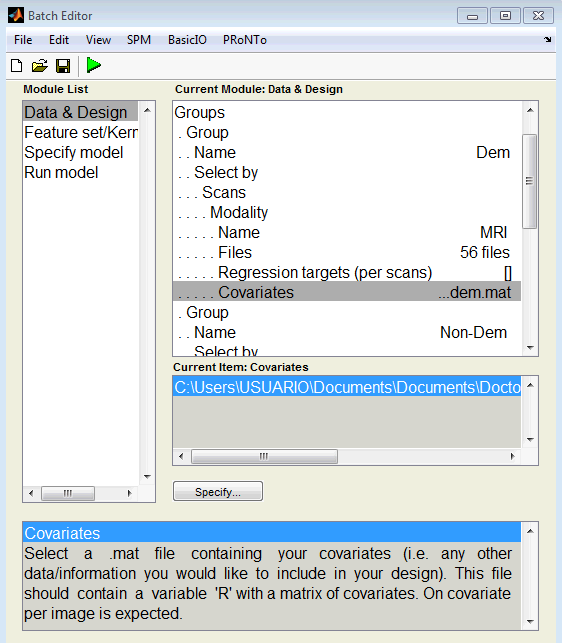
\includegraphics[scale=0.6]{images/Tutorial/confounds/covariates_batch.png}
	\caption{Data and design module in {\tt matlabbatch}. }
	\label{fig:covariates_batch}
	\end{figure}
				
		
	\end{itemize}
	
	\item In the `Masks' field, add a new modality and provide the same modality name, `MRI'; and select the `mergedsmwrc1\_mask\_01' mask available of the Oasis dataset. The name of the modality here has to be exactly the same as in `Modalities', otherwise it will not work;
	
	%checar aqui
	
	\item Leave the `HRF overlap' and the `HRF delay' fields as default;
	
	\item In the `Review' field, select `Yes' if you would like to review your data and design in a separate window. Otherwise, leave as it is, i.e. `No'.


\end{itemize}

%------------------------------------------------------------

\subsection{Feature set / Kernel}

\begin{itemize}
	\item Click on the `Feature set / Kernel' option on PRoNTo's {\tt matlabbatch} menu (see Figure \ref{fig:batchFeature} in Chapter \ref{sec:Block_design_fMRI_dataset});
	
	\item With `Load PRT.mat' field selected, click on the `Dependency' button to associate the `PRT.mat' file created in the previous `Data \& Design' step (Figure \ref{fig:batchDependency}) or click on the `Select files' button to browse where `PRT.mat' file was saved;
	
	
    \item Provide a name to the `Feature/kernel' set, e.g. `svmDem-NonDem';
	
	\item Add one modality and select the modality name with the `Dependency' button\footnote{Or type it in manually, `MRI', but the name needs to be {\it exactly} the same as the one specified in the `Data \& Design' module.}(Data \& Design:Mod\#1 name);
	
		\begin{itemize}
	
	\item In the `Scans/Conditions' field , select the `All scans' option;
	
	\item In the `Voxels to include' field, select `All voxels' option, this means we are not entering an additional second-level mask;
	
	\item In the `Detrend' field, select `Polynomial detrend' option with order 1;
	
	\item In the `Scale input scans' field, select `No scaling' option;
	
	\item Leave `Load Atlas' as default. After all these steps, the batch editor should look similar to the one in Figure \ref{fig:feature_batch};
	
	\begin{figure}[h!]
	\centering
		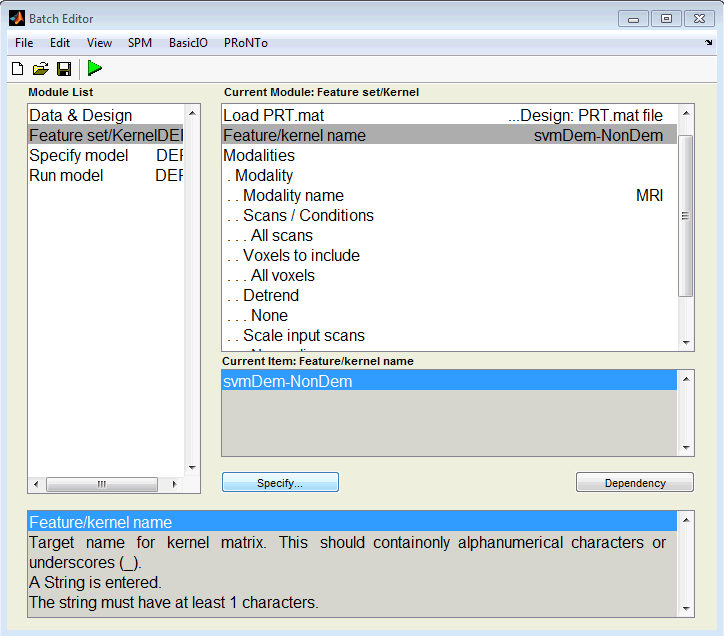
\includegraphics[scale=0.55]{images/Tutorial/confounds/feature_batch.png}
	\caption{Feature set / Kernel module. Selected parameters in the Modality option.}
	\label{fig:feature_batch}
\end{figure}
	
	\end{itemize}
	
	\item Leave the `Generate Multiple Kernels' and the `Use one kernel per modality' fields as default.
	

\end{itemize}

%--------------------------------------------------------

\subsection{Specify model}

\begin{itemize}

\item Click on the `Specify model' option on PRoNTo's {\tt matlabbatch} menu (see Figure \ref{fig:batchSpecifyModel} in Chapter \ref{sec:Block_design_fMRI_dataset});
	
\item With `Load PRT.mat' field selected, click on the `Dependency' button to associate the `PRT.mat' file created in the previous `Feature set / Kernel' step or click on the `Select files' button to browse where `PRT.mat' file was saved;

\item Provide a name to the model, e.g. `SVM';   

\item Leave the `Use kernels' field as it is, i.e. `Yes';    

\item Select the feature set name with the `Dependency' button\footnote{or write it {\it exactly} as previously defined in the `Feature set / Kernel' module (option `Feature set/Kernel: Feature/kernel name'), here `svmDem-NonDem'.};    
	
	\item Select the `Classification' model type:
	
		\begin{itemize}
		
		\item Add 2 new classes;
		
		\item For Class (1) write `Demented' on the name field and add one group. Select the group name from the `Data \& Design' module (`Data \& Design:Group\#1 name') with the `Dependency' button\footnote{Or write it {\it exactly}, as previously defined in the Data \& Design' module, here `Dem'}. Similarly, for Class (2) write `Non-Demented' on the name field and add the group created in the `Data \& Design' module, `Non-Dem';	
		
		\item In the `Subjects' field of the Group 1, type `1:56'. This will instruct the program to use all the 56 scans, i.e. from scan 1 to scan 56. Similarly, in the `Subjects' field of the Group 2, type `1:39'.

		\end{itemize}			
		
	\item In the `Machine' field:
	
	\begin{itemize}
	\item Select the `SVM Classification' option;	
	
	\item Leave the `Optimize hyper-parameter' field as it is, i.e. `No';
	
	\item Leave the `Soft-margin hyper-parameter' field as it is, i.e. `1';
	
	\item Leave the `Cross validation type for hyper-parameter optimization' field as it is, i.e. `Leave one subject out';  
	
	
	\end{itemize}
	
	\item In the `Cross-validation type' field, select `Leave one subject out' option;
	
	\item Leave the `Include all scans' field as it is, i.e. `No';

	\item In the `Data operations' field:
	
		\begin{itemize}
		\item  Leave the `Mean centre features' field as it is, i.e. `Yes'; 
				
		\item  Click on the `Other Operations' button, choose `Select operations', `New Operation' and select the `Regress out covariates (subject level)' option from the list. After all these steps, the batch editor should look similar to the one in Figure \ref{fig:model_batch};
		\end{itemize}
		
	\begin{figure}[h!]
	\centering
		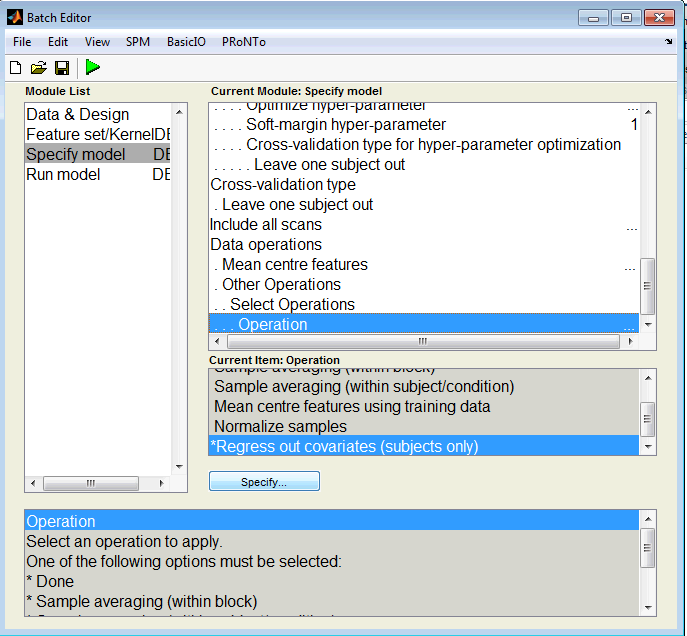
\includegraphics[scale=0.6]{images/Tutorial/confounds/model_batch.png}
	\caption{Data and design module in {\tt matlabbatch}. }
	\label{fig:model_batch}
	\end{figure}
	
\end{itemize}

%----------------------------------------------------------

\subsection{Run model}

\begin{itemize}

    \item Click on the `Run model' option on PRoNTo's {\tt matlabbatch} menu (see Figure \ref{fig:batchRun} in Chapter \ref{sec:Block_design_fMRI_dataset});
    
   	\item  With `Load PRT.mat' field selected, click on the `Dependency' button to associate the `PRT.mat' file created in the previous `Specify model' step;

    \item Select the model name from the `Specify model' module with the `Dependency' button\footnote{or write it {\it exactly} as previously defined in the `Specify model' module, here `SVM'};
    
    \item In the field `Do permutation test?', leave as it is, i.e. `No permutation test' 

\end{itemize}


\subsection{Display weights}

\begin{itemize}
	
	\item In PRoNTo's main window, click on `Display weights' and select the `PRT.mat' file. This will open the `Model interpretation' window.
	
	\item By clicking on `Model', SVM, an image will appear in the `Weights map' box; and to show the `Anatomical img' you have to load an anatomical image for reference. A template image can be found in SPM's canonical folder (`single\_subj\_T1` file). The final window will look similar to the one shown in the Figure \ref{fig:weights_map}.
	
\begin{figure}[h!]
	\centering
		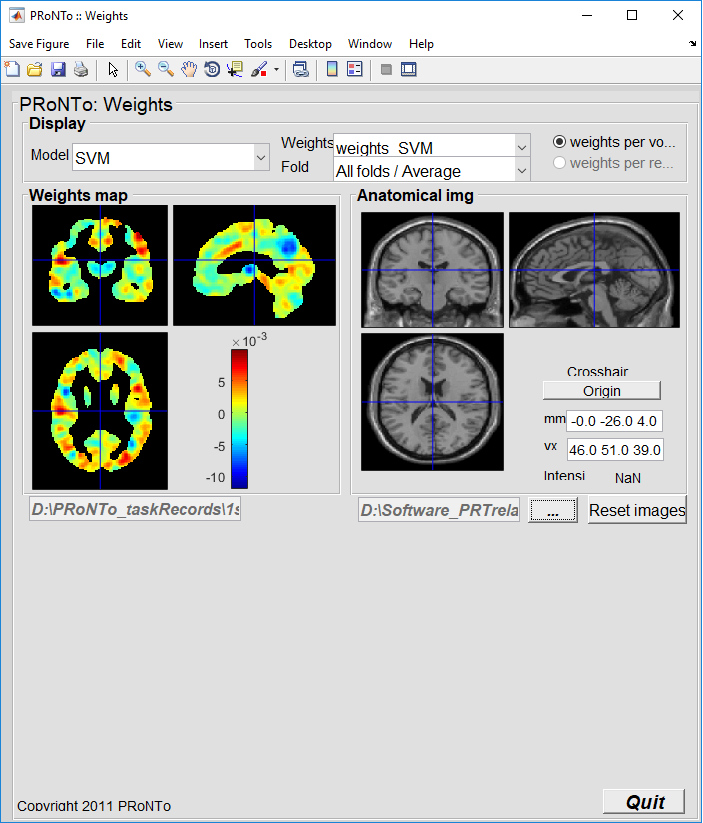
\includegraphics[height=10cm]{images/Tutorial/classification/prt_weights_covariates}
	\caption{Weights map}
	\label{fig:weights_map}
\end{figure}

	
\end{itemize}

